\section{Módulo de conexión}
\label{sec:arqMuphic}
\gotrev{Última revisión hecha el 20-06-2012}

El módulo de conexión se encarga de lanzar los módulos de análisis y/o el de composición, según la demanda del usuario. Para ello, debe ejecutar los correspondientes programas asociados a cada módulo, de tal forma que la vista de despliegue es tal y como muestra la Figura~\ref{fig:muphic-deploy-diagram}.\\


		\begin{figure}[!htbp]
		\centering
		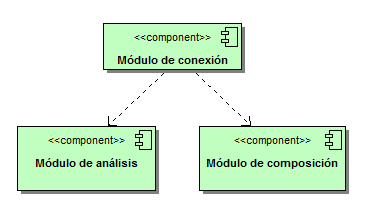
\includegraphics[scale=0.6]{graphics/muphic-deploy-diagram.png}
		\caption{Diagrama de despliegue del módulo de interconexión}
		\label{fig:muphic-deploy-diagram}
		\end{figure}
		
Es aquí donde surge el principal problema de que la aplicación sea multiplataforma, ya que distintos sistemas operativos, como Windows o los basados en UNIX, proponen distintas maneras de lanzar archivos ejecutables. Para solventar estos problemas, se han concentrado las consiguientes diferencias del código para cada sistema operativo en la clase \emph{Launcher}, como se ve en la Figura~\ref{fig:muphic-class-diagram}.\\

		\begin{figure}[!htbp]
		\centering
		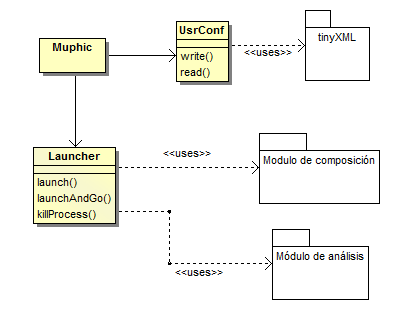
\includegraphics[scale=0.6]{graphics/muphic-class-diagram.png}
		\caption{Diagrama de clases del módulo de interconexión}
		\label{fig:muphic-class-diagram}
		\end{figure}
		
La clase Launcher ofrece funcionalidad para ejecutar una aplicación interrumpiendo la ejecución en curso (\emph{Launcher::launch()}), o bien en paralelo (\emph{Launcher::launchAndGo()}), así como para detener la ejecución de un programa lanzado (\emph{Launcher::killProcess()}). De esta forma, la totalidad del resto del código del proyecto se ha realizado sin preocuparse de la plataforma de ejecución, delegando de Launcher siempre que era necesario realizar operaciones propias de cada sistema operativo.\\

En la Figura~\ref{fig:muphic-sec-diagram} se muestra un ejemplo de ejecución del módulo, en el que se ejecutan tanto el módulo de análisis como el de composición.\\

		\begin{figure}[!htbp]
		\centering
		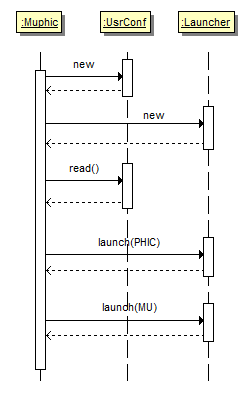
\includegraphics[scale=0.6]{graphics/muphic-sec-diagram.png}
		\caption{Diagrama de flujo del módulo de interconexión}
		\label{fig:muphic-sec-diagram}
		\end{figure}
		
Cabe destacar en esta sección el uso de la clase \emph{UsrConf}, encargada de administrar el archivo de configuración del completo proceso de análisis y composición. Este archivo de configuración es el que permite la ``comunicación'' entre los distintos módulos del sistema. Está estructurado en forma de XML y contiene tanto los parámetros necesarios para la ejecución del módulo de análisis como los necesarios para la ejecución del módulo de composición (vistos en la Sección~\ref{chap:guiauso}). Contiene también la información de la ruta destino de la composición. De forma adicional, permite indicar qué módulo se debe ejecutar, de forma que se puede ejecutar únicamente uno de los dos módulos o los dos a la vez. La clase \emph{UsrConf} ofrece funcionalidad para escribir y leer (ya sea en su totalidad o la parte relativa a un único módulo) el archivo XML.\\

\section{Interfaz Gráfica}
\label{sec:arqgui}

\torev{Pendiente de Primera Revisión}

La interfaz gráfica de la aplicación es la encargada de aunar todas las funcionalidades del sistema en una única aplicación. Se ocupa de la creación del archivo de configuración necesario para la ejecución de los distintos módulos, así como de facilitar el acceso a los resultados del análisis y la composición.\\

Para su diseño se ha usado el quit de desarrollo Qt (Apéndice~\ref{sec:Qt}), por ser multiplataforma y a estar en sí misma orientada a móviles, facilitando así una futura movilización del sistema a máquinas portátiles. La versión de la librería usada está aplicada al lenguaje de programación C++, gracias a lo cual se ha podido reusar gran parte del código implementado en el resto del sistema, como son las clases UsrConf (encargada de almacenar la configuración de los módulos, como se vio en la Sección~\cite{sec:arqMuphic}), y el paquete de representación de figuras (las clases \emph{Figures} y derivadas, vistas en la Sección~\ref{sec:representacionFiguras}. La interfaz, como se ve en en los requisitos (Sección~\ref{sec:requisitos}), debe ser capaz tanto de lanzar el módulo de conexión como de mostrar el resultado del análisis y la partitura de la pieza musical compuesta, así como reproducir dicha pieza generada.\\

Mientras que para mostrar el análisis y reproducir música se podrá utilizar los mismos recursos ofrecidos por la librería Qt, para mostrar las partituras será necesario hacer uso del visor de archivos gráficos predeterminado del sistema (en concreto se usa el formato de archivos xhtml, por facilidad de uso en las diferentes plataformas a las que está orientada la aplicación). Es por ello que se utiliza también la clase \emph{Launcher} anteriormente explicada, que en esta ocasión lanzará cada aplicación en paralelo a la interfaz gráfica, permitiendo así detener la ejecución de módulos externos si el usuario considera que su período de actividad ha sido excesivo.\\

La siguiente sección analizará con detalle la implementación de las partes más importantes de esta interfaz.

\subsection{Vista de implementación}

La aplicación sigue la estructura básica de una interfaz diseñada sobre Qt, con un controlador encargado de manejar los eventos (\emph{QMainWindow}) y una estructura que se encarga de actualizar la parte gráfica (\emph{MuphicUI}), como se ve en la Figura~\ref{fig:gui-class-diagram}.\\

		\begin{figure}[!htbp]
		\centering
		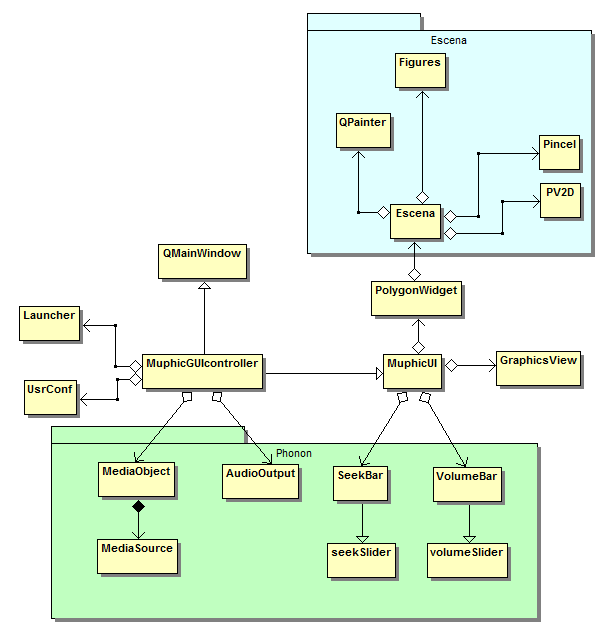
\includegraphics[scale=0.6]{graphics/gui_diagrama_clases.png}
		\caption{Diagrama de flujo del módulo de interconexión}
		\label{fig:gui-class-diagram}
		\end{figure}

Para mostrar la imagen seleccionada como entrada se usa un elemento propio de la librería Qt (\emph{GraphicsView}), mientras que para la visualización del resultado final de un análisis recién efectuado, se usa una clase propia: \emph{PolygonWidget}. Su estructura, como muestra la Figura~\ref{fig:gui-class-diagram}, consta de un elemento principal, la \emph{Escena}, encargada de administrar el marco de dibujo y sus contenidos. Ella hará uso de la estructura de representación de Figuras para cargar la imagen recién analizada y pintarla en el marco designado, gracias a la clase pintora \emph{QPainter} proporcionada por la librería. Con ella, y utilizando la clase auxiliar \emph{Pincel} (que facilita el pintado de líneas y arcos aproximados por rectas), mostrará por pantalla la escena cargada, proporcionando al usuario una visión fiel del análisis realizado.\\

Por otro lado, para la reproducción de audio se hace uso de una librería compaginable con Qt: Phonon (Apéndice~\ref{sec:Phonon}). Esta librería se encarga de cargar así como de iniciar, parar y modificar el transcurso de la reproducción de una pieza musical. El uso de esta librería, que soporta archivos de audio tales como wav o mp3, pero no midi, obliga a que el módulo de reproducción produzca una salida acorde a los formatos que esta librería es capaz de reproducir.

\subsection{Vista de despliegue}

A diferencia de otros apartados, donde la totalidad de los elementos externos se incluyen en el despliegue del módulo, en este caso se exigirá como requisito de instalación a los usuarios de sistemas UNIX el tener instalados en sus máquinas anfitrionas tanto la librería Qt como la librería adicional Phonon, para ahorrar espacio en el producto final. Se encuentran detalladas estas librerías en la Sección~\ref{sec:reqinstalacion}.\\

En la versión para sistemas Windows, por proporcionarse un instalable y no el código fuente, no será necesario que exista ninguna librería instalada en el sistema.\\